
%% bare_conf.tex
%% V1.3
%% 2007/01/11
%% by Michael Shell
%% See:
%% http://www.michaelshell.org/
%% for current contact information.
%%
%% This is a skeleton file demonstrating the use of IEEEtran.cls
%% (requires IEEEtran.cls version 1.7 or later) with an IEEE conference paper.
%%
%% Support sites:
%% http://www.michaelshell.org/tex/ieeetran/
%% http://www.ctan.org/tex-archive/macros/latex/contrib/IEEEtran/
%% and
%% http://www.ieee.org/

%%*************************************************************************
%% Legal Notice:
%% This code is offered as-is without any warranty either expressed or
%% implied; without even the implied warranty of MERCHANTABILITY or
%% FITNESS FOR A PARTICULAR PURPOSE! 
%% User assumes all risk.
%% In no event shall IEEE or any contributor to this code be liable for
%% any damages or losses, including, but not limited to, incidental,
%% consequential, or any other damages, resulting from the use or misuse
%% of any information contained here.
%%
%% All comments are the opinions of their respective authors and are not
%% necessarily endorsed by the IEEE.
%%
%% This work is distributed under the LaTeX Project Public License (LPPL)
%% ( http://www.latex-project.org/ ) version 1.3, and may be freely used,
%% distributed and modified. A copy of the LPPL, version 1.3, is included
%% in the base LaTeX documentation of all distributions of LaTeX released
%% 2003/12/01 or later.
%% Retain all contribution notices and credits.
%% ** Modified files should be clearly indicated as such, including  **
%% ** renaming them and changing author support contact information. **
%%
%% File list of work: IEEEtran.cls, IEEEtran_HOWTO.pdf, bare_adv.tex,
%%                    bare_conf.tex, bare_jrnl.tex, bare_jrnl_compsoc.tex
%%*************************************************************************

% *** Authors should verify (and, if needed, correct) their LaTeX system  ***
% *** with the testflow diagnostic prior to trusting their LaTeX platform ***
% *** with production work. IEEE's font choices can trigger bugs that do  ***
% *** not appear when using other class files.                            ***
% The testflow support page is at:
% http://www.michaelshell.org/tex/testflow/



% Note that the a4paper option is mainly intended so that authors in
% countries using A4 can easily print to A4 and see how their papers will
% look in print - the typesetting of the document will not typically be
% affected with changes in paper size (but the bottom and side margins will).
% Use the testflow package mentioned above to verify correct handling of
% both paper sizes by the user's LaTeX system.
%
% Also note that the "draftcls" or "draftclsnofoot", not "draft", option
% should be used if it is desired that the figures are to be displayed in
% draft mode.
%
\documentclass[conference]{IEEEtran}
% Add the compsoc option for Computer Society conferences.
%
% If IEEEtran.cls has not been installed into the LaTeX system files,
% manually specify the path to it like:
% \documentclass[conference]{../sty/IEEEtran}

% Some very useful LaTeX packages include:
% (uncomment the ones you want to load)


% *** MISC UTILITY PACKAGES ***
%
\usepackage{ifpdf}
% Heiko Oberdiek's ifpdf.sty is very useful if you need conditional
% compilation based on whether the output is pdf or dvi.
% usage:
% \ifpdf
%   % pdf code
% \else
%   % dvi code
% \fi
% The latest version of ifpdf.sty can be obtained from:
% http://www.ctan.org/tex-archive/macros/latex/contrib/oberdiek/
% Also, note that IEEEtran.cls V1.7 and later provides a builtin
% \ifCLASSINFOpdf conditional that works the same way.
% When switching from latex to pdflatex and vice-versa, the compiler may
% have to be run twice to clear warning/error messages.




% *** CITATION PACKAGES ***
%
%\usepackage{cite}
% cite.sty was written by Donald Arseneau
% V1.6 and later of IEEEtran pre-defines the format of the cite.sty package
% \cite{} output to follow that of IEEE. Loading the cite package will
% result in citation numbers being automatically sorted and properly
% "compressed/ranged". e.g., [1], [9], [2], [7], [5], [6] without using
% cite.sty will become [1], [2], [5]--[7], [9] using cite.sty. cite.sty's
% \cite will automatically add leading space, if needed. Use cite.sty's
% noadjust option (cite.sty V3.8 and later) if you want to turn this off.
% cite.sty is already installed on most LaTeX systems. Be sure and use
% version 4.0 (2003-05-27) and later if using hyperref.sty. cite.sty does
% not currently provide for hyperlinked citations.
% The latest version can be obtained at:
% http://www.ctan.org/tex-archive/macros/latex/contrib/cite/
% The documentation is contained in the cite.sty file itself.




% *** GRAPHICS RELATED PACKAGES ***
%
\ifpdf
  \usepackage[pdftex]{graphicx}
  % declare the path(s) where your graphic files are
  \graphicspath{{../pdf/}{../jpeg/}{img/}}
  % and their extensions so you won't have to specify these with
  % every instance of \includegraphics
  \DeclareGraphicsExtensions{.pdf,.jpeg,.png}
\else
  % or other class option (dvipsone, dvipdf, if not using dvips). graphicx
  % will default to the driver specified in the system graphics.cfg if no
  % driver is specified.
  \usepackage[dvips]{graphicx}
  % declare the path(s) where your graphic files are
  \graphicspath{{../eps/}}
  % and their extensions so you won't have to specify these with
  % every instance of \includegraphics
  \DeclareGraphicsExtensions{.eps}
\fi% graphicx was written by David Carlisle and Sebastian Rahtz. It is
% required if you want graphics, photos, etc. graphicx.sty is already
% installed on most LaTeX systems. The latest version and documentation can
% be obtained at: 
% http://www.ctan.org/tex-archive/macros/latex/required/graphics/
% Another good source of documentation is "Using Imported Graphics in
% LaTeX2e" by Keith Reckdahl which can be found as epslatex.ps or
% epslatex.pdf at: http://www.ctan.org/tex-archive/info/
%
% latex, and pdflatex in dvi mode, support graphics in encapsulated
% postscript (.eps) format. pdflatex in pdf mode supports graphics
% in .pdf, .jpeg, .png and .mps (metapost) formats. Users should ensure
% that all non-photo figures use a vector format (.eps, .pdf, .mps) and
% not a bitmapped formats (.jpeg, .png). IEEE frowns on bitmapped formats
% which can result in "jaggedy"/blurry rendering of lines and letters as
% well as large increases in file sizes.
%
% You can find documentation about the pdfTeX application at:
% http://www.tug.org/applications/pdftex





% *** MATH PACKAGES ***
%
\usepackage[cmex10]{amsmath}
% A popular package from the American Mathematical Society that provides
% many useful and powerful commands for dealing with mathematics. If using
% it, be sure to load this package with the cmex10 option to ensure that
% only type 1 fonts will utilized at all point sizes. Without this option,
% it is possible that some math symbols, particularly those within
% footnotes, will be rendered in bitmap form which will result in a
% document that can not be IEEE Xplore compliant!
%
% Also, note that the amsmath package sets \interdisplaylinepenalty to 10000
% thus preventing page breaks from occurring within multiline equations. Use:
\interdisplaylinepenalty=2500
% after loading amsmath to restore such page breaks as IEEEtran.cls normally
% does. amsmath.sty is already installed on most LaTeX systems. The latest
% version and documentation can be obtained at:
% http://www.ctan.org/tex-archive/macros/latex/required/amslatex/math/

% ADDED BY BOLSTER
\usepackage{amssymb}




% *** SPECIALIZED LIST PACKAGES ***
%
%\usepackage{algorithmic}
% algorithmic.sty was written by Peter Williams and Rogerio Brito.
% This package provides an algorithmic environment fo describing algorithms.
% You can use the algorithmic environment in-text or within a figure
% environment to provide for a floating algorithm. Do NOT use the algorithm
% floating environment provided by algorithm.sty (by the same authors) or
% algorithm2e.sty (by Christophe Fiorio) as IEEE does not use dedicated
% algorithm float types and packages that provide these will not provide
% correct IEEE style captions. The latest version and documentation of
% algorithmic.sty can be obtained at:
% http://www.ctan.org/tex-archive/macros/latex/contrib/algorithms/
% There is also a support site at:
% http://algorithms.berlios.de/index.html
% Also of interest may be the (relatively newer and more customizable)
% algorithmicx.sty package by Szasz Janos:
% http://www.ctan.org/tex-archive/macros/latex/contrib/algorithmicx/
\usepackage{algpseudocode}




% *** ALIGNMENT PACKAGES ***
%
%\usepackage{array}
% Frank Mittelbach's and David Carlisle's array.sty patches and improves
% the standard LaTeX2e array and tabular environments to provide better
% appearance and additional user controls. As the default LaTeX2e table
% generation code is lacking to the point of almost being broken with
% respect to the quality of the end results, all users are strongly
% advised to use an enhanced (at the very least that provided by array.sty)
% set of table tools. array.sty is already installed on most systems. The
% latest version and documentation can be obtained at:
% http://www.ctan.org/tex-archive/macros/latex/required/tools/


\usepackage{mdwmath}
\usepackage{mdwtab}
% Also highly recommended is Mark Wooding's extremely powerful MDW tools,
% especially mdwmath.sty and mdwtab.sty which are used to format equations
% and tables, respectively. The MDWtools set is already installed on most
% LaTeX systems. The lastest version and documentation is available at:
% http://www.ctan.org/tex-archive/macros/latex/contrib/mdwtools/


% IEEEtran contains the IEEEeqnarray family of commands that can be used to
% generate multiline equations as well as matrices, tables, etc., of high
% quality.


%\usepackage{eqparbox}
% Also of notable interest is Scott Pakin's eqparbox package for creating
% (automatically sized) equal width boxes - aka "natural width parboxes".
% Available at:
% http://www.ctan.org/tex-archive/macros/latex/contrib/eqparbox/





% *** SUBFIGURE PACKAGES ***
%\usepackage[tight,footnotesize]{subfigure}
% subfigure.sty was written by Steven Douglas Cochran. This package makes it
% easy to put subfigures in your figures. e.g., "Figure 1a and 1b". For IEEE
% work, it is a good idea to load it with the tight package option to reduce
% the amount of white space around the subfigures. subfigure.sty is already
% installed on most LaTeX systems. The latest version and documentation can
% be obtained at:
% http://www.ctan.org/tex-archive/obsolete/macros/latex/contrib/subfigure/
% subfigure.sty has been superceeded by subfig.sty.



%\usepackage[caption=false]{caption}
%\usepackage[font=footnotesize]{subfig}
% subfig.sty, also written by Steven Douglas Cochran, is the modern
% replacement for subfigure.sty. However, subfig.sty requires and
% automatically loads Axel Sommerfeldt's caption.sty which will override
% IEEEtran.cls handling of captions and this will result in nonIEEE style
% figure/table captions. To prevent this problem, be sure and preload
% caption.sty with its "caption=false" package option. This is will preserve
% IEEEtran.cls handing of captions. Version 1.3 (2005/06/28) and later 
% (recommended due to many improvements over 1.2) of subfig.sty supports
% the caption=false option directly:
\usepackage[caption=false,font=footnotesize]{subfig}
%
% The latest version and documentation can be obtained at:
% http://www.ctan.org/tex-archive/macros/latex/contrib/subfig/
% The latest version and documentation of caption.sty can be obtained at:
% http://www.ctan.org/tex-archive/macros/latex/contrib/caption/




% *** FLOAT PACKAGES ***
%
%\usepackage{fixltx2e}
% fixltx2e, the successor to the earlier fix2col.sty, was written by
% Frank Mittelbach and David Carlisle. This package corrects a few problems
% in the LaTeX2e kernel, the most notable of which is that in current
% LaTeX2e releases, the ordering of single and double column floats is not
% guaranteed to be preserved. Thus, an unpatched LaTeX2e can allow a
% single column figure to be placed prior to an earlier double column
% figure. The latest version and documentation can be found at:
% http://www.ctan.org/tex-archive/macros/latex/base/



%\usepackage{stfloats}
% stfloats.sty was written by Sigitas Tolusis. This package gives LaTeX2e
% the ability to do double column floats at the bottom of the page as well
% as the top. (e.g., "\begin{figure*}[!b]" is not normally possible in
% LaTeX2e). It also provides a command:
%\fnbelowfloat
% to enable the placement of footnotes below bottom floats (the standard
% LaTeX2e kernel puts them above bottom floats). This is an invasive package
% which rewrites many portions of the LaTeX2e float routines. It may not work
% with other packages that modify the LaTeX2e float routines. The latest
% version and documentation can be obtained at:
% http://www.ctan.org/tex-archive/macros/latex/contrib/sttools/
% Documentation is contained in the stfloats.sty comments as well as in the
% presfull.pdf file. Do not use the stfloats baselinefloat ability as IEEE
% does not allow \baselineskip to stretch. Authors submitting work to the
% IEEE should note that IEEE rarely uses double column equations and
% that authors should try to avoid such use. Do not be tempted to use the
% cuted.sty or midfloat.sty packages (also by Sigitas Tolusis) as IEEE does
% not format its papers in such ways.





% *** PDF, URL AND HYPERLINK PACKAGES ***
%
\usepackage{url}
% url.sty was written by Donald Arseneau. It provides better support for
% handling and breaking URLs. url.sty is already installed on most LaTeX
% systems. The latest version can be obtained at:
% http://www.ctan.org/tex-archive/macros/latex/contrib/misc/
% Read the url.sty source comments for usage information. Basically,
% \url{my_url_here}.





% *** Do not adjust lengths that control margins, column widths, etc. ***
% *** Do not use packages that alter fonts (such as pslatex).         ***
% There should be no need to do such things with IEEEtran.cls V1.6 and later.
% (Unless specifically asked to do so by the journal or conference you plan
% to submit to, of course. )


% correct bad hyphenation here
\hyphenation{op-tical net-works semi-conduc-tor}

%%%%%%%%%%%%%%%%%%%%%%%%%%%%%%%%%%%
% BOLSTER PACKAGES FOR DEV PERIOD %
%%%%%%%%%%%%%%%%%%%%%%%%%%%%%%%%%%%
\usepackage{booktabs}
\usepackage{hyperref}
\usepackage{todonotes}
\presetkeys%
    {todonotes}%
    {inline,backgroundcolor=yellow}{}

\graphicspath{{../../../Figures/}{./figures/}}


\begin{document}
%
% paper title
% can use linebreaks \\ within to get better formatting as desired
\title{Mobility for Trust Assessment in Autonomous Underwater MANETs}


% author names and affiliations
% use a multiple column layout for up to three different
% affiliations
\author{\IEEEauthorblockN{Andrew Bolster}
\IEEEauthorblockA{Department of Electrical Engineering and Electronics\\
University of Liverpool\\
Liverpool, UK\\
Email: bolster@liv.ac.uk}
\and
\IEEEauthorblockN{Alan Marshall}
\IEEEauthorblockA{Department of Electrical Engineering and Electronics\\
University of Liverpool\\
Liverpool, UK\\
Email: alan.marshall@liv.ac.uk}
}

% use for special paper notices
\IEEEspecialpapernotice{Pages: 9, Deadline: 25/3}




% make the title area
\maketitle


\begin{abstract}
%\boldmath

\emph{Relevant sections from the \href{http://www.ene.unb.br/mass2016/}{CFP} art: Key Mgmt \& Trust Establishment; Robotic Networks; Vehicular Networks \& Protocols; Location Based Services; Mobility Managment}

\todo{Do this last}

\end{abstract}
% no keywords

% For peer review papers, you can put extra information on the cover
% page as needed:
% \ifCLASSOPTIONpeerreview
% \begin{center} \bfseries EDICS Category: 3-BBND \end{center}
% \fi
%
% For peerreview papers, this IEEEtran command inserts a page break and
% creates the second title. It will be ignored for other modes.
\IEEEpeerreviewmaketitle



\section{Introduction}

In the majority of Trusted autonomous mobile network implementations, a free space RF communications protocol such as 802.11 is used as the source of all information about the trustworthy operation of the network.
By their nature, such implementations rely on relatively high bandwidth, low noise, low latency, and high channel occupancy where contention is tolerable.
In contrast; in underwater environments, communications is sparse, delayful, noisy, and very prone to destructive contention.
Therefore, observations of the communications processes used to assess trust occur much less frequently, with much greater error (noise) and delay than is experienced in terrestrial RF MANETS.
In addition to the communications challenges, other considerations such as command and control isolation, as well as power and locomotive limitations, and the increasing drive towards the use of teams of smaller, cheaper, almost disposable autonomous underwater vehicles (AUVs), particularly in defense, ecological and petrochemical fields, present unique threats against trust management. 

Trust Management Frameworks (TMFs) provide information to assist the estimation of future states and actions of nodes operating as teams, groups or networks. 
This information is used to optimize the performance of a team against malicious, selfish, or defective misbehaviour by one or more nodes.
Previous research has established the advantages of implementing communications-based TMFs in terrestrial, 802.11 based MANETs, particularly in terms of preventing selfish operation in collaborative systems \cite{Li2007}, and maintaining throughput in the presence of malicious actors \cite{Buchegger2002}. 
Most current TMFs use a single type of observed communication action to derive trust assessments, typically successfully delivered or forwarded packets. 
These observations then inform future decisions of individual nodes, for example, route selection \cite{Li2008}.

Recent work has demonstrated the use of a number of metrics to form a ``vector'' of trust. The Multi-parameter Trust Framework for MANETs (MTFM) \cite{Guo11}, uses a range of communications metrics beyond packet delivery/loss rate (PLR) to assess trust. This vectorized trust also allows a system to detect and identify the tactics being used to undermine or subvert trust. 
This method as been previously applied to the marine space, comparing against a selection of existing communications TMFs \cite{Bolster2015} showing that MTFM is more effective at detecting misbehaviours in sparse communications environments. 

This paper investigates the application of these communication-based Trust methodologies to the physical domain, to assess the viability of using the motion and mobility of nodes within a team to detect and potentially identify malicious or failing operation within a cohort.
This is accomplished by looking specifically at operations within the three dimensions of the underwater space.

In Section~\ref{sec:mobility}, we review the current applications and mobility patters of collaborative AUV operations, and the current state-of-the-art in underwater localisation techniques.
In Section~\ref{sec:tmfs}, we discuss the use of TMFs in the terrestrial space and their applicability to marine operations in general. 
In Section~\ref{sec:exp}, we design a series of simulations, hypotheses, and tests to assess the detection and identification capabilities of three potential physical metrics for trust assessment.


\section{AUV Mobility and Localisation}\label{sec:mobility}

The use and applications of Autonomous Underwater Vehicles (AUVs) has undergone a great expansion in recent times; current applications and considerations are given in Table~\ref{tab:auv_apps} (summarised from \cite{Jalving2003}\cite{andThen}).
For the purposes of this exploratory case we do not model the hydrodynamics of the control surfaces of the AUVs, however we do model axial drag as a resistive inertial force.

\begin{table}[h]
  \caption{Applications of AUVs} \label{tab:auv_apps}
  \begin{center}
    \setlength{\tabcolsep}{8pt}
    \begin{tabular}{lcc}
      \toprule
      \bottomrule
    \end{tabular}
    \setlength{\tabcolsep}{6pt}
  \end{center}
\end{table}

\subsection{AUV operations and deployments}

\todo{I have something for this but can't lay my hands on it at the moment; TLDR the used cubic port protection / littoral survey model used isn't perfect but its a reasonable analogue}
\todo{\emph{For Chapter} Look at redoing this with other mobilities (particularly distributed lawnmower)}

\subsection{Localisation Technologies}

Given the subsurface nature of most AUV operations, terrestrial localisation techniques such as GPS are unavailable (below $\approx 20cm$ depth). 
However, a range of alternative techniques are used to maintain spacial awareness to a high degree of accuracy in the underwater environment.
\subsubsection{Long baseline (LBL)}
Long-baseline localisation systems use a series of static surface/cable networked acoustic transponders to provide coordinated beacons and (usually) GPS-backed relative location information to local subsurface users. 
Such systems can be accurate to less that $0.1m$ or better in ideal deployments and are regularly used in controlled autonomous survey environments such as harbour patrol operations where the deployment area is bounded. 
However, the initial setup and deployment required in advance of any AUV operation makes LBL difficult to utilise in unbounded or contended areas.
LBL systems can also be deployed on mobile surface platforms in the area (ships or buoys for example), but these applications put significant computational pressure on the end-point AUV and have greatly reduced accuracy compared to ideal deployments\cite{Matos1999}.
\subsubsection{Doppler Velocity Log (DVL)}
Doppler logging involves the emission of directed acoustic ``pings'' that reflect off sea bed/surface interfaces that, when received back on the craft with multi-beam phased array acoustic transducers can measure both the absolute depth/altitude (z-axis) of the craft and through directional Doppler shifting, the relative (xy-translative) motion of the craft since the ping.
While classical DVL was highly sensitive to shifting currents in the water column, advances in the development of Acoustic Doppler Current Profiling has turned that situation on it's head, enabling the compensation-for and measurement-of water currents down to the sub-meter level\cite{Snyder2010}.
\subsubsection{Inertial Navigation Systems (INS)}
Inertial navigation systems use gyroscopic procession to observe the relative acceleration of a mobile platform.
This reference-relative monitoring is particularly useful in the underwater environment, as it detects the motion of AUVs as they are carried by the water itself.
Bias Drift is a significant problem for INS systems operating over longer (hundreds of metres) distances, as they usually have some minimal amount of directional bias, that incurs a cumulative effect over time without assistance.
Several sensor synthesis processes have been demonstrated which combine information from INS along with DVL data to improve localisation into the sub-decimeter level\cite{Jalving2003}\cite{Liu2014}.

\subsubsection{Simultaneous Location and Mapping (SLAM)}
Simultaneous Location and Mapping is the process of iteratively developing a feature-based model of an environment, and to use the relative movement within that modeled environment to obtain estimates of absolute positioning.
SLAM has been most well developed in the contexts of either visual-based inspection using cameras, or LIDAR-style distance triangulation, however the same principles have been successfully applied using marine sonar readings, providing sub-meter accuracy, feature-relative localisation information that is (for the most part) environmentally agnostic\cite{Williams2000}.


\section{Trust Management Frameworks}\label{sec:tmfs}

Trust Management Frameworks (TMFs) are used to improve the efficiency, security, and reliability of decentralized and distributed autonomous systems. 
Techniques have been developed for high-speed, uncontended environments such as terrestrial 802.11 MANETs. 
However, these do not perform well in sparse / harsh environments such as those found in Underwater Acoustic Networks (UANs), where network nodes experience significant and variable delays, comparatively low data rates, large contention periods, and considerable multi-path artefacts.\cite{Bolster2015} 
\todo{Not sure how much detail to go into in this section; this paper isn't about the formation of trust from metrics, it's about the assessment of metrics at all}

\section{Experimental Design}\label{sec:exp}

\subsection{Physical Metrics}

Three physical metrics are selected to encompass the relative distributions and activities of nodes within the network; Inter-node Distance Deviation (INDD), Inter-node Heading Deviation (INHD), and Node Speed. 
These metrics encapsulate the relative distributions of position and velocity of a particular observed node, optimising for the detection of outlying or deviant behaviour within the fleet.

Given that local nodes within the team are aware of the reported positions and velocities of their neighbours, it is believed that this is a reasonable initial set of metrics to establish the usefulness of physical metrics of trust assessment.

Additional metric constructions may be more suitable for certain contexts, platforms or operations, however these were selected in collaboration with UK DSTL and NATO CMRE as suitable, generic, assessments, viable on most current platforms in most current deployment schemes.

Conceptually, INDD is a measure of the average spacing of an observed node with respect to its neighbours. INHD is a similar approach with respect to node orientation.

\begin{align}
  INDD_{i,j} &= \frac{|P_j - \sum_x \frac{P_x}{N}|}{\frac{1}{N}\sum_x \sum_y{|P_x - P_y| (\forall x \neq y)}}\\
  INHD_{i,j} &= \hat{v} \vert v= V_j - \sum_x{\frac{V_x}{N}}\\
  V_{i,j} &= |V_j|
\end{align}

Where $i$ and $j$ are indices denoting the current observer node and the current observed node respectively; $x$ is a summation index representing other nodes in the observers region of concern; $P{j}$ is the $[x,y,z]$ absolute position of the observed node (relative to some coordinated origin point agreed upon at launch) and $V{j}$ is the $[x,y,z]$ velocity of the observed node.

Thus, the metric vector used for the physical-trust assessment from one observer node to a given target node is;

\begin{equation}
  X_{i,j}=\{\text{INDD}_{i,j}, \text{INHD}_{i,j},, V_{i,j}\}
  \label{eq:phys_vector}
\end{equation}
At each time-step, each node will have a separate $X$ assessment vector for each node it has observed in that time. 
Ergo the fleet or team as a whole will have $N\times N$ assessment vectors at each timestep.

\subsection{Physical Misbehaviours}
Misbehaviours in the communications space is heavily investigated area in MANETs \cite{Konate2011}\cite{Wang2009}\cite{Chen2014a}\cite{Mitchell2014}, but attacks and misbehaviours in the physical space are far less explored. 
Both in terrestrial and underwater contexts, as MANET applications expand and become increasingly \emph{de rigueur}, the impacts of physical or operational misbehaviour become increasingly relevant. 
As in the communications space, the primary drivers of any ``misbehaviour'' come under two general categories; selfish operation or malicious subterfuge.
Autonomous MANETs in general rely (or are at least, most effective) when all nodes operate fairly, be that in terms of their bandwidth sharing, energy usage, routing optimality or other factors. 
Physically, if a node is being ``selfish'', it may preferentially move to the edge of a network to minimise it's dynamic work allocation, or depending on it's intent, may insert itself into the centre of a network to maximise it's ability to capture, monitor, and manipulate traffic going across the network. 
In the context of a secure operation (or one that's assumed to be secure), the opportunity for capturing a legitimate node and replacing it with a modified clone.
Assuming a highly capable outside actor and a multi-channel communications opportunity, there is even the possibility of a node appearing to ``play along'' with the crowd that occasionally breaks rank to route internal transmissions to a outside agent.
In the underwater context this may mean an AUV following the rest of a team along a survey path and occasionally ``breaking surface'' to communicate to a malicious controller.
Alternatively, if an inserted node is not totally aware of a given mission parameter, such as a particular survey or waypointing path, it may simply follow along, hoping not to be noticed.

In all these cases, such behaviour involves some element of behaving differently from the rest of the team, however, there are other cases where such individual ``deviance'' is observed; where a node is in some kind of mechanical ``failure state''.
In the underwater context, this could be damage to the drive-train or navigation systems, causing it to lag behind or consistently drift off course. 
An ideal physical trust management system would be able to differentiate between both ``malicious'' behaviours and ``failing'' behaviours.

To investigate this hypothesis, we create two ``bad'' behaviours; one ``malicious'', where a cloned node is unaware of the missions' survey parameters and attempts to ``hide'' among the fleet, and a ``failing'' node, with an impaired drive train, increasing the drag force on the nodes movement.
These two behaviours are designated \emph{Shadow} and \emph{SlowCoach} respectively.

\subsection{Simulation Background}

Simulations were conducted using a Python based simulation framework, SimPy \cite{Mueller2003SimPy}, with a network stack built upon AUVNetSim \cite{Miquel2008}, with transmission parameters taken from and validated against \cite{Stojanovic2007} and \cite{Stefanov2011}.
For the purposes of this paper, this network is used for the dissemination of node location information, assuming suitable compression of internally assumed location data compressed into one 4096 bit acoustic data frame.
Node kinematics are based on REMUS 100 Autonomous Underwater Vehicles, based on limits and core characteristics given in \cite{Mcewen2001}, \cite{Milgram2001} and \cite{Samad2011}.

These limits are given in Table~\ref{tab:mobility_sysconstraints}
\begin{table}[h]
  \caption{REMUS 100 Mobility Constraints as applied in simulation} \label{tab:mobility_sysconstraints}
  \begin{center}
    \setlength{\tabcolsep}{8pt}
    \begin{tabular}{lcc}
      \toprule
      Parameter & Unit & Value \\
      \midrule
      Length & $m$ & 5.5\\
      Diameter & $m$ & 0.5\\
      Mass & $kg$ & 37 \\ 
      Max Speed & $ms^{-1}$ & 2.5\\
      Cruising Speed & $ms^{-1}$ & 1.5\\
      Max X-axis Turn & $^{\circ} s^{-1}$ & 4.5\\
      Max Y-axis Turn & $^{\circ} s^{-1}$ & 4.5\\
      Max Z-axis Turn & $^{\circ} s^{-1}$ & 4.5\\
      Axial Drag Coefficient ($c_d$) & NA & 3\\
      Cross Section Area & $m^2$ & 0.13\\

      \bottomrule
    \end{tabular}
    \setlength{\tabcolsep}{6pt}
  \end{center}
\end{table}

\subsection{Node Control Modelling}

Simple Boidean flocking \cite{Reynolds1987a} is used in addition to the guiding Waypointing behaviour to provide a collision-avoidance capability.
This consists of three heuristic rules; Cohesion, Repulsion and Alignment, and are shown visually in~\ref{fig:boids} and mathematically below.
\begin{itemize}
  \item Cohesion
    \begin{equation}
      F_{j,C}= F_A\left(p_j, \frac{1}{N}\sum\limits_{\forall i \ne j}^N{p_i}, d_{max}\right)
    \end{equation}
  \item Repulsion
    \begin{equation}
      F_{j,R}= \sum\limits_{\forall i \ne j}^N F_R\left(p_j, p_i, d_{max}) \big| d_{max}>\|p_i-p_j\|\right)
    \end{equation}
  \item Alignment
    \begin{equation}
      F_{j,CA}= \frac{1}{N}\cdot\left(\sum\limits_{\forall i \ne j}^N \hat{v_i}\right) 
    \end{equation}
\end{itemize}
where $F$'s are force-vectors applied to the internal guidance of the AUV, 
Where $F_A$ is a scaled vector attraction function, and $F_R$ is an equivalent repulsion function
\begin{align}
  F_A(p^a, p^i)=&(\widehat{p^a-p^i}) \times \frac{|p^a-p^i|}{d}\\
  F_R(p^r, p^i)=&(\widehat{p^i-p^r}) \times \frac{|p^r-p^i|}{d}
\end{align}

\begin{figure*}
  \centering
  \subfloat[Cohesion]{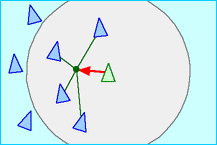
\includegraphics[width=0.3\textwidth]{flocking_cohesion}}
  \subfloat[Repulsion]{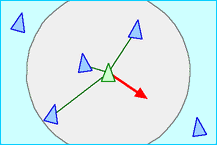
\includegraphics[width=0.3\textwidth]{flocking_separation}}
  \subfloat[Alignment]{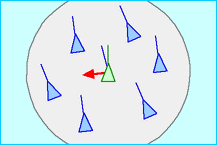
\includegraphics[width=0.3\textwidth]{flocking_alignment}}
  \caption{Visual representation of the basic Boidean collision avoidance rules used}
  \label{fig:boids}
\end{figure*}



\subsection{Standards of Accuracy}

The key question of this paper is to assess the advantages and disadvantages of utilising trust from the physical domain. 

It is important to clarify what is meant by ``effective'' in this case; the ``effectiveness'' of any trust assessment framework is taken as consisting of several parts.

\begin{enumerate}
  \item the \emph{accuracy} of detection and identification of a particular misbehaviour
  \item the \emph{timeliness} of such detections
  \item the \emph{complexity} of such analysis, including any specific training required
  \item the \emph{commonality} of the results of any detections between perspectives (also termed ``isomorphism'' of results)
\end{enumerate}

In this case we are particularly interested in the accuracy of detection and identification of malicious / failing behaviours, and as such are looking at three key characteristics of accuracy; true detection accuracy (what percentage of ``bad'' behaviours are detected at all); false positive rates (what percentage of ``control'' behaviours are detected as being ``bad''); and misidentification rates (how many instances of one bad behaviour are mischaracterised as the other and vie versa.

As such we have three primary questions to answer to establish if these metrics are useful:
\begin{itemize}
  \item How accurate are these metrics in being able to easily differentiate between Normal and Abnormal behaviours in terms of True-Positive and False-Positive rates?
  \item What differentiation of response, if any, is there between the stated abnormal behaviours?
  \item Can a simple classification be built to characterise these differentiations of response, and what is it's True-Positive/False-Positive accuracy?
\end{itemize}


\subsection{Analysis Workflow}
Having established the metrics under investigation, $MANY$ simluation runs are executed for each scenario (i.e.\ one node ``Maliciously'' following the fleet with no mission information, one ``Failing'' node with simulated drivetrain issues, and one baseline control scenario where all nodes are behaving appropriatly.
Eash of these simulated missions last for $duration$, matching realistic deployment times based on current MOD/NATO operations\cite{Bolster2014a}\cite{SomethingElse}.

\subsubsection{Metric Cleaning}
In order to assess the viability of using the previously discussed metrics for behaviour assessment, the raw motion paths recorded by the simulation are fed into an analysis pipeline\footnote{We do not currently deal with the case where nodes maliciously ``fake'' their location}.
This pipeline initially 

\begin{figure}
  \begin{algorithmic}
    \ForAll{m in M}
      \ForAll{t}
      \State $d_{i,j}^{m,t} = x_{i,j}^{m,t} - \frac{\sum_k x_{i,k}^{m,t}}{|M|}$
      \State $\alpha_{i,j}^{m,t} = | \frac{d_{i,j}^{m,t}}{\sigma{d_{i,j}^{m,t}}}|$
      \EndFor
    \EndFor
  \end{algorithmic}
  \caption{Numerical Analysis Pipeline for Metric Value Assessment}
  \label{fig:workflow}
\end{figure}

Where $i$ and $j$ are indices denoting the current observer node and the current observed node respectively; $x$ is a summation index representing other nodes in the observers region of concern; $X$ is the vector of metrics from~\ref{eq:phys_vector}; $d$ is an intermediate value of the distance of a given observation from the mean, and $\alpha$ is a resulting normalised response value in terms of it's deviation from the mean.

\subsubsection{Behaviour Detection and Classification}
\todo{This is going to be a bit of a black box while I work out what works automatically; previous versions simply looked at the ``Highest Deviator'', and while that still works in terms of detection, it's not massively useful in terms of Identification. Could be that in terms of the criteria posed above (simplicity of computation) that using the basic toolkits, we can't do it, however I'd rather not have every single paper I do in my career have half a page explaining the abstract operation of Gray Theory\dots}

One simple behaviour detection is to apply Dixon's Q-test \cite{Dean1951} to the resultant $\sum\alpha$ values for each node for each metric for each run  a) establish if a ``misbheaving node'' exists in a given run, and b) identify that misbehaving node. 

\todo{If you need padding at the end, explain Dixon}

For our initial investigation we will use a Confidence Interval of $95\%$.
Our initial hypothesis is that by using observations of the previously stated physical metrics, that we will be able to detect and identify misbehaviours.
Within that context, this Confidence Interval indicates that we would expect only a $5\%$ chance that any run or node identified using the Q-test to \emph{not} be a misbehaving run/node.

Further, due to the range of metrics available to us, by applying the Q-test on a per-metric basis, we can use the ``votes'' of each metric as a simplified consensus classifier.
\todo{There's got to be a better phrase than ``consensus''\dots}
This classifier may allow us to characterise some aspect of a given misbehaviour in terms of metrics it heavily impacts, and those that are less affected.

This can then be augmented by taking the residual deviation of $\sum\alpha_{i}$ to generate a ``confidence'' score of a given node being an outlier in a given metric;

\begin{equation}
  C_{i}^{m} = \Sigma_t\sigma_{i}^m * \frac{N-1}{\sum_{x\neq i}{\Sigma_t\sigma_{x}^m}}\label{eq:confidence}
\end{equation}


\subsubsection{Operational Performance Metrics}
\todo{``How do we measure the impact of a bad-physical-behaviour on the operational success/efficiency of the fleet overall?''. We have these numbers already in terms of energy use/efficiency of locomotion, cumulative distance covered, mean time to targets, etc, just need to wrap some words around it}

\section{Results and Discussion}
\begin{figure*}
  \centering
  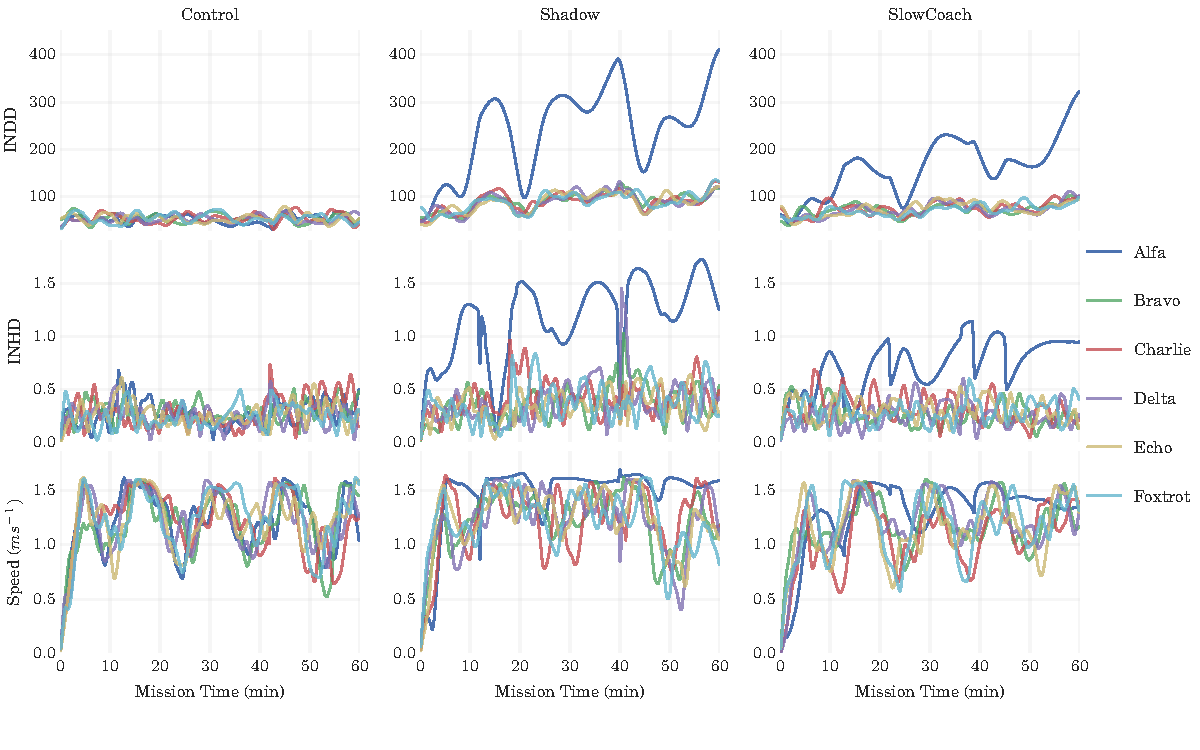
\includegraphics[width=0.8\textwidth]{Metric_Values}
  \caption{Observed Metric Values for one simulation of each behaviour ($x_{i,j}^{m,t}$ from Fig.~\ref{fig:workflow})}
\end{figure*}

\begin{figure*}
  \centering
  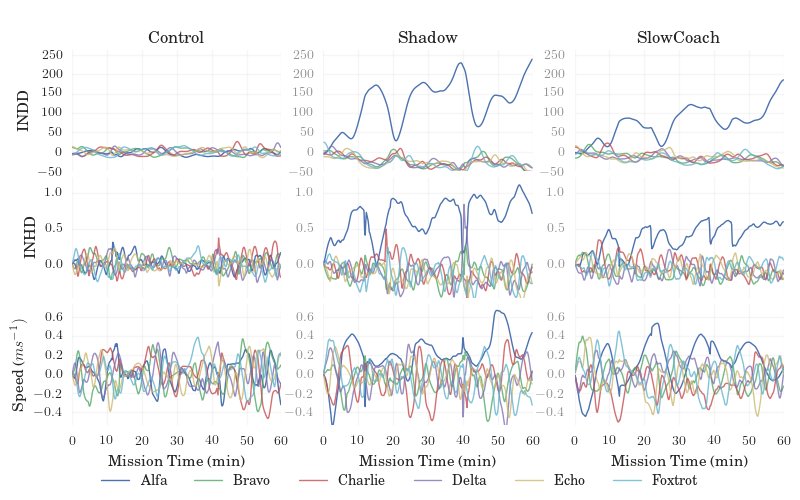
\includegraphics[width=0.8\textwidth]{Metric_Deviation}
  \caption{\emph{Unnecessary but included for draft discussion} Observed Metric Values for one simulation of each behaviour ($d_{i,j}^{m,t}$ from Fig.~\ref{fig:workflow})}
\end{figure*}

\begin{figure*}
  \centering
  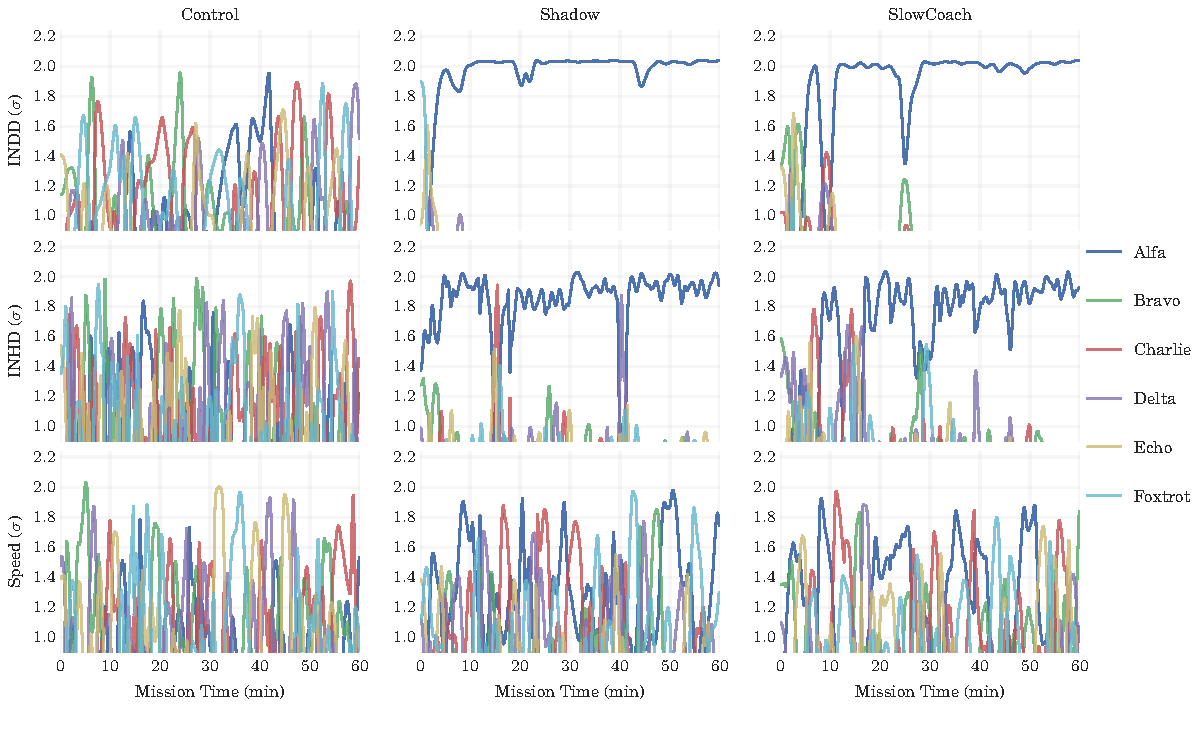
\includegraphics[width=0.8\textwidth]{Metric_Sigma_Deviance}
  \caption{Observed Metric Values for one simulation of each behaviour ($\alpha_{i,j}^{m,t}$ from Fig.~\ref{fig:workflow})}
\end{figure*}

\begin{figure*}
  \centering
  \subfloat[INDD]{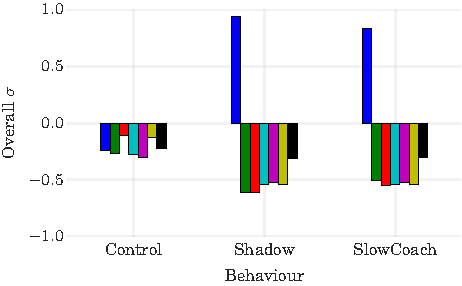
\includegraphics[width=0.6\linewidth]{summedsigmabar_INDD}}\\
  \subfloat[INHD]{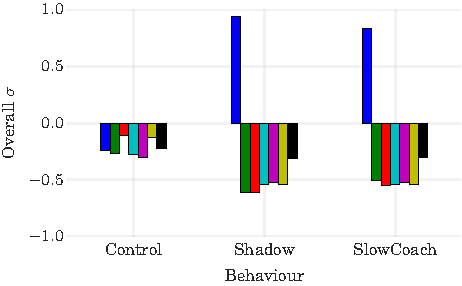
\includegraphics[width=0.6\linewidth]{summedsigmabar_INDD}}\\
  \subfloat[Speed]{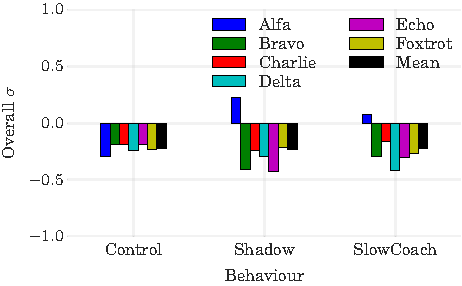
\includegraphics[width=0.6\linewidth]{summedsigmabar_Speed}}
  \caption{\emph{VERY Draft; don't get pissy!}: Per-Node-Per-Run $\sum\alpha/T$}
\end{figure*}

\subsection{Detection of Misbehaviours}

\subsection{Identification of Misbehaviours}
\todo{The below table is whats going to be used to condense all the ugly above into something processable across many runs (and most importatly, blind runs)}
\begin{table}[h]
  \caption{Metric Confidence Responses for known behaviours~\eqref{eq:confidence}}
  \centering
  \begin{tabular}{lrrr}
    \toprule
    metric &      INDD &      INHD &     Speed \\
    var       &           &           &           \\
    \midrule
    Shadow    &  3.802935 &  3.191642 &  1.867909 \\
    SlowCoach &  4.227141 &  2.773664 &  1.509357 \\
    Tail      &  3.874741 &  3.652717 &  2.155030 \\
    Waypoint  &  0.920183 &  0.966642 &  0.958920 \\
    \bottomrule
  \end{tabular}
\end{table}

\subsection{Impacts of Misbehaviour on operational performance}

\section{Conclusion}
In this paper we have demonstrated that with current and on-the-horizon underwater localisation techniques, that in certain mobility models, that a set of relatively simple geometric abstractions (INHD, INDD, and Speed), between nodes as part of an Underwater MANET can be used as a Trust Assessment and Establishment metric.

We show, using a basic cubic survey mobility model built upon a Boidian collision prevention behaviour that in a simulated underwater environment, the outputs of these metrics can be used to detect and differentiate between example malicious behaviour and potential failure states.

This verification further supports the assertions the authors have made previously in \cite{Bolster2014}  that it is practical to extend Trust protocols such as Multi-parameter Trust Framework for MANETS (MTFM)\cite{Guo2012} to include metrics and observations from the physical domain as well as those from the communication domain. 
This combination of physical and ``logical'' information would further support the decentralised and distributed establishment of observation based Trust, reducing the significant 


% conference papers do not normally have an appendix


% use section* for acknowledgement
\section*{Acknowledgment}

The Authors would like to thank the DSTL/DGA UK/FR PhD Programme for their support during this project, as well as NATO CMRE for their advice and assistance.

\bibliographystyle{IEEEtran}
% argument is your BibTeX string definitions and bibliography database(s)
\bibliography{IEEEabrv,refs}

% that's all folks
\end{document}


% An example of a floating figure using the graphicx package.
% Note that \label must occur AFTER (or within) \caption.
% For figures, \caption should occur after the \includegraphics.
% Note that IEEEtran v1.7 and later has special internal code that
% is designed to preserve the operation of \label within \caption
% even when the captionsoff option is in effect. However, because
% of issues like this, it may be the safest practice to put all your
% \label just after \caption rather than within \caption{}.
%
% Reminder: the "draftcls" or "draftclsnofoot", not "draft", class
% option should be used if it is desired that the figures are to be
% displayed while in draft mode.
%
%\begin{figure}[!t]
%\centering
%\includegraphics[width=2.5in]{myfigure}
% where an .eps filename suffix will be assumed under latex, 
% and a .pdf suffix will be assumed for pdflatex; or what has been declared
% via \DeclareGraphicsExtensions.
%\caption{Simulation Results}
%\label{fig_sim}
%\end{figure}

% Note that IEEE typically puts floats only at the top, even when this
% results in a large percentage of a column being occupied by floats.


% An example of a double column floating figure using two subfigures.
% (The subfig.sty package must be loaded for this to work.)
% The subfigure \label commands are set within each subfloat command, the
% \label for the overall figure must come after \caption.
% \hfil must be used as a separator to get equal spacing.
% The subfigure.sty package works much the same way, except \subfigure is
% used instead of \subfloat.
%
%\begin{figure*}[!t]
%\centerline{\subfloat[Case I]\includegraphics[width=2.5in]{subfigcase1}%
%\label{fig_first_case}}
%\hfil
%\subfloat[Case II]{\includegraphics[width=2.5in]{subfigcase2}%
%\label{fig_second_case}}}
%\caption{Simulation results}
%\label{fig_sim}
%\end{figure*}
%
% Note that often IEEE papers with subfigures do not employ subfigure
% captions (using the optional argument to \subfloat), but instead will
% reference/describe all of them (a), (b), etc., within the main caption.


% An example of a floating table. Note that, for IEEE style tables, the 
% \caption command should come BEFORE the table. Table text will default to
% \footnotesize as IEEE normally uses this smaller font for tables.
% The \label must come after \caption as always.
%
%\begin{table}[!t]
%% increase table row spacing, adjust to taste
%\renewcommand{\arraystretch}{1.3}
% if using array.sty, it might be a good idea to tweak the value of
% \extrarowheight as needed to properly center the text within the cells
%\caption{An Example of a Table}
%\label{table_example}
%\centering
%% Some packages, such as MDW tools, offer better commands for making tables
%% than the plain LaTeX2e tabular which is used here.
%\begin{tabular}{|c||c|}
%\hline
%One & Two\\
%\hline
%Three & Four\\
%\hline
%\end{tabular}
%\end{table}


% Note that IEEE does not put floats in the very first column - or typically
% anywhere on the first page for that matter. Also, in-text middle ("here")
% positioning is not used. Most IEEE journals/conferences use top floats
% exclusively. Note that, LaTeX2e, unlike IEEE journals/conferences, places
% footnotes above bottom floats. This can be corrected via the \fnbelowfloat
% command of the stfloats package.


